\chapter{Épée et bocle -- généralités}


\section{Introduction}


La bocle est un petit bouclier circulaire.
Cette combinaison était très populaire car la bocle est peu encombrante et peut facilement être transportée avec l'épée.

La prise naturelle de l'épée est celle dite de "prise marteau".
\index{prise!marteau}
Toutefois cette prise n'est pas très bien adaptée au mouvement exécuté en épée-bocle (que ce soit en I.33 ou en Liegniczer) car elle ne permet pas d'être fort sur certains liages ou d'exécuter certains mouvements.
Ainsi nous utilisons plutôt la "prise sabre", où le pouce (plus exactement la pulpe) est calé dans l'angle entre le quillon et la fusée (voir l'exercice~\ref{épée-bocle:I33:ex:krucke-liage})~\cite{fuhrmann:dijon:I33_liage:2015}.
\index{prise!sabre}
Cette prise est aussi naturelle sur des épées de type I.33 dont la poignée était courte : dans ce cas le bas de la main est bien maintenu par le pommeau.
\index{prise!en croix}
Finalement certains mouvements se feront avec le pouce placé sur la croix formée par la fusée et les quillons (nous l'appellerons "prise en croix"), comme à l'épée longue.
Cette prise permet de donner des coups horizontaux très rapidement et d'être ferme en garde haute (bœuf).
L'idéal est donc de pouvoir passer rapidement de la prise en croix à la prise sabre : cela peut se faire en utilisant le pouce pour faire pivoter l'épée dans la main~\footnotemark{} ; dans ce cas on peut aussi avoir une prise sabre où le pouce se trouve légèrement sur la gauche de l'angle.
\footnotetext{Cela peut être plus difficile à faire avec des gants et Roland Fuhrmann conseille de ne pas en porter pour travailler la technique~\cite{fuhrmann:dijon:I33_liage:2015}.}
% voir technique 2 de Fuhrmann

La bocle n'est pas un bouclier efficace : elle est trop petite pour dévier efficacement, et même si l'on parvient à arrêter un coup l'adversaire pourra facilement passer derrière.
Le principal intérêt de la bocle est de pouvoir protéger le bras d'arme, qui peut donc être étendu plus loin que si la bocle ne le protégeait pas (ce principe s'applique surtout au I.33 et à Liegniczer).
Il faut tenir la bocle relativement loin du corps afin de couvrir une plus grande surface (figure~\ref{épée-bocle:fig:bocle-cone}).
Un second intérêt à la bocle est de s'en servir pour frapper l'adversaire et pour contrôler ses mains (et donc sa bocle et/ou son épée).


\begin{figure}[ht]
	\centering
	\subfloat[Bocle éloignée.]{\includegraphics{epee_bocle/bocle_cone_loin}}
	\hspace{1cm}
	\subfloat[Bocle proche.]{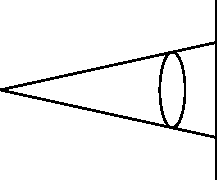
\includegraphics{epee_bocle/bocle_cone_proche}}
	\caption{Cônes de protections pour une bocle tenue loin et près.}
	\label{épée-bocle:fig:bocle-cone}
\end{figure}


\begin{exercice}[Défendre la main]

\D tend le bras droit devant lui et place sa main gauche près de sa main droite. 
\A essaie de toucher la main droite de \D qui ne peut se défendre qu'avec la main gauche.

Cet exercice travaille le fait de placer sa bocle du côté de l'épée adverse et de réagir vite pour l'intercepter.

% Source : Arthur.
\end{exercice}


% fluidité
\begin{exercice}[Changements de garde]

Passer d'une garde à une autre en intercalant une frappe à chaque fois.
Chercher à être fluide.
\end{exercice}


\begin{exercice}[Couper la main]

\begin{enumerate}
	\item \A porte une attaque lente à \D, qui se défend simplement.
	\item Si une partie du corps de \A n'est pas protégée, alors \D amène son épée pour le mettre en évidence.
\end{enumerate}

\A peut enchaîner les frappes (en laissant le temps à \D de réagir pour mettre en évidence une éventuelle erreur).
Le but n'est pas d'aller vite mais de vérifier si la position est correcte.

Au début \D peut se concentrer uniquement sur la main d'arme de \A en faisant peu de mouvements, puis quand \A commence à avoir l'habitude \D peut chercher d'autres cibles et bouger légèrement.
\end{exercice}


\section{Gardes}


Nous listons dans cette section toutes les gardes quelque soit leur origine car nous utiliserons un vocabulaire commun dans les sections qui suivent.


\begin{garde}[Crosse – \emph{Krucke}]
\index{krucke}
\index{garde!épée-bocle!krucke}

Dans la garde de la crosse (all. \emph{Krucke}, ang. \emph{crutch}), les mains sont placées face au visage, la pointe de l'épée vers le bas, la bocle couvrant la main d'arme.
\end{garde}


Cette garde est très hermétique et permet de dévier les estocs bas.

